\documentclass[a4paper,11pt,dvipdfmx]{ujarticle}
\usepackage{float}
\usepackage{graphicx}
\usepackage{url}
\input{layout}

\title{日本におけるデジタル化の現状}
\author{G58489-2025 向井梨茉}

\begin{document}

\maketitle 

\section{デジタル競争率ランキング}

国際経営開発研究所(IMD)の調査\cite{IMD}によると,日本のデジタル競争力のランキングは図\ref{fig:競争率}に示すように、
調査対象64カ国中,総合で28位,知識分野で25位となっている。

\begin{figure}[htbp]
    \centering
    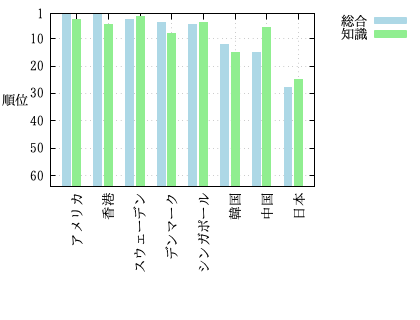
\includegraphics{fig31.png}
    \caption{デジタル競争率ランキング(64カ国中)}\label{fig:競争率}
\end{figure}



% 本文(1)
%  参考文献の参照: \cite{}
%  図番号の参照: \ref{}、
% を使う
% 文献データベースのキーワードは oecd と imd
% になっている.

% 図の挿入
% \includegraphics{}
% を
% \begin{figure}[htbp]
% \end{figure}
% で囲み
% \caption{}
% で図のタイトルを入れる.
% \label{}
% を使って図番号が参照できるようにする
% また,
% \centering
% で図が中央に来るようにする

% ーーー
\section{ブロードバンドの整備状況}

OECDによるブローバンド回線の普及に関する調査\cite{oecd}によると、表\ref{tbl:加入者数}に示すように,
日本における100人あたりの光ファイバー回線の加入者数は29.0で,
韓国,スウェーデン,
ノルウェーに続いて第4位となっている。

\begin{table}[htbp]
    \centering
    \caption{光ファイバー回線の加入者数}
    \label{tbl:加入者数}

    \begin{tabular}{|c|l|r|}
        \hline
        順位 & 国名 & 加入者数 \\
        \hline
        1位 & 韓国 & 38.2 \\
        \hline
        2位 & スウェーデン & 31.9 \\
        \hline
        3位 & ノルウェー & 29.5 \\
        \hline
        4位 & 日本 & 29.0 \\
        \hline
        5位 & アイスランド & 28.8 \\
        \hline
        6位 & スペイン & 27.3 \\
        \hline
        7位 & ポルトガル & 25.1 \\
        \hline
        8位 & ニュージーランド & 23.6 \\
        \hline
        9位 & リトアニア & 22.3 \\
        \hline
        10位 & フランス & 21.2 \\
        \hline
    \end{tabular}
\end{table}

\section{考察}

\begin{itemize}
    \item 韓国の光ファイバー加入率が1番多い。
    \item 日本の光ファイバー加入率は4位であり、1位との差は約15%である。
    \item デジタル競争率ランキングはアメリカが1位である。
    \item 日本は中国よりも競争率ランキングは低いためあげていく必要がある。
\end{itemize}





        % \begin{tabular}
% \end{tabular}    
% による表の記述を 
% \begin{table}[htbp]
% \end{table}
% で囲み
% \caption{}
% で表のタイトルを入れる.
% \label{}
% を使って表番号が参照できるようにする
% また,
% \centering
% で表が中央に来るようにする

% ーーー
% 見出し(3)
% 考察
%
% \begin{itemize}
% \end{itemize}
% を使って箇条書きで記述する

% ここに参考文献が入る
%
\bibliographystyle{junsrt}
\bibliography{exercise.bib}
\
\end{document}